
%(BEGIN_QUESTION)
% Copyright 2010, Tony R. Kuphaldt, released under the Creative Commons Attribution License (v 1.0)
% This means you may do almost anything with this work of mine, so long as you give me proper credit

Calculate the flow rate necessary (in units of gallons per minute) to create exactly 0 PSI gauge pressure at the throat of this venturi, and also calculate the (ideal) pressure at the third gauge.  Assume water with a mass density ($\rho$) of 1.951 slugs per cubic foot:

$$\includegraphics[width=15.5cm]{i00444x01.eps}$$

Furthermore, determine what will happen to the pressure at the throat if the flow rate increases beyond this rate, assuming all other factors remain unchanged?

\underbar{file i00444}
%(END_QUESTION)





%(BEGIN_ANSWER)

$Q$ = 7550.29 GPM

\vskip 10pt

If the flow rate increases beyond 7550.29 GPM, the pressure at $P_2$ will decrease further, creating a vacuum.

%(END_ANSWER)





%(BEGIN_NOTES)


%INDEX% Physics, dynamic fluids: Bernoulli's equation

%(END_NOTES)


